%%%%%%%%%%%%%%%%%%%%%%%%%%%%%%%%%%%%%%%%%
% Template for describing the test procedure specification.
% structure and annotations are quoted from IEEE Std 829-1998
%%%%%%%%%%%%%%%%%%%%%%%%%%%%%%%%%%%%%%%%%
\starttps{wp21-cr-ts01-webas01-tps02}


\noindent\textbf{Test design specification reference: \refexpdoc{wp21-cr-ts01-webas01-tds01}}\\
\noindent\textbf{Test case specification reference: \refexpdoc{wp21-cr-ts01-webas01-tcs02}}\\
\noindent\textbf{Test log identifier: \refexpdoc{wp21-cr-ts01-webas01-tl02}}

%Purpose:
%To specify the steps for executing a set of test cases or, more generally, the steps used to analyze a software
%item in order to evaluate a set of features.

%Outline:
%A test procedure specification shall have the following structure:
%a) Test procedure specification identifier.
%b) Purpose;
%c) Special requirements;
%d) Procedure steps.
%The sections shall be ordered in the specified sequence. Additional sections, if required, may be included at
%the end. If some or all of the content of a section is in another document, then a reference to that material
%may be listed in place of the corresponding content. The referenced material must be attached to the test
%procedure specification or available to users of the procedure specification.
%Details on the content of each section are contained in the following subclauses.


\subsubsection{Purpose}
%Describe the purpose of this procedure. If this procedure executes any test cases, provide a reference for each
%of them.
%In addition, provide references to relevant sections of the test item documentation (e.g., references to usage
%procedures).
The purpose of this test is to evaluate whether the checkpointing and restarting mechanism perform correctly by using the SAP WebAS as the test application.

\subsubsection{Procedure Steps}
%Include the following steps as applicable.

\paragraph{Installation}
The test requires a proper Linux system without further modifications. Furthermore, the standard SAP WebAS 6.40 has to be installed on this Linux machine. The setup of the checkpointing and restarting functionalities is described under setup.

\paragraph{Log}
%Describe any special methods or formats for logging the results of test execution, the incidents observed, and
%any other events pertinent to the test (see Clauses 9 and 10).
The startup output of the SAP WebAS is available on the command line. If the system is up an running, the graphical user interfaces of the SAP WebAS can be used to evaluate whether the system behaves correctly.

\paragraph{Set Up}
%Describe the sequence of actions necessary to prepare for execution of the procedure.
First, the checkpointing and restarting mechanism needs to be installed. This is done as described for \refexpdoc{wp21-cr-ts01-webas01-tps01}. Therefore, we do not repeat these steps here. The SAP WebAS is installed following the standard SAP procedure. As this is a rather long description and specific to SAP, we do not describe this process here.

\paragraph{Start}
The start of the WebAS is simple.
\begin{lstlisting}
#su benadm
# whoami
benadm
# startsap
\end{lstlisting}

\paragraph{Proceed}
The proceed process consists of using the generated checkpoint and then restarting the application.

\paragraph{Measure}
%Describe how the test measurements will be made (e.g., describe how remote terminal response time is to be
%measured using a network simulator).
The measurement is the check whether the system response is normal during the start up as well as after the checkpointing and restarting of the SAP WebAS.

Thus, the start up should be as follows:
\begin{lstlisting}
#su benadm
# whoami
benadm
# startsap

Checking BEN Database
------------------------------
 ABAP Database is not available via R3trans

Checking BEN Database
------------------------------

Starting SAP-Collector Daemon
------------------------------
16:08:12 08.11.2007   LOG: Effective User Id is root
******************************************************
* This is Saposcol Version COLL 20.93 640 - AMD/Intel 
x86_64 with Linux, PL:159, Nov 23 2006
* Usage:  saposcol -l: Start OS Collector
*         saposcol -k: Stop  OS Collector
*         saposcol -d: OS Collector Dialog Mode
*         saposcol -s: OS Collector Status
* The OS Collector (PID 5980) is already running .....
******************************************************
 saposcol already running
 Running /usr/sap/BEN/SYS/exe/run/startdb
Trying to start database ...
Log file: /usr/sap/BEN/benadm/startdb.log
BEN database started
/usr/sap/BEN/SYS/exe/run/startdb completed successfully

Checking BEN Database
------------------------------
 ABAP Database is running

Starting SAP Instance DVEBMGS19
------------------------------
 Startup-Log is written to /usr/sap/BEN/benadm/startsap_
 DVEBMGS19.log
 Instance on host bfssrv05 started
\end{lstlisting}
The user should be able to login to the system as shown in Figures~\ref{fig:SAP1} and \ref{fig:SAP2}.

\begin{figure}[h!]
    \centerline{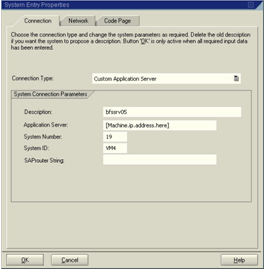
\includegraphics[scale=0.80]{../experiments/wp21-cr/ts01/SAP1.png}}
    \caption{\label{fig:SAP1}Login for the SAP WebAS.}
\end{figure}
\begin{figure}[h!]
    \centerline{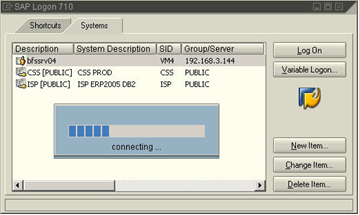
\includegraphics[scale=0.80]{../experiments/wp21-cr/ts01/SAP2.png}}
    \caption{\label{fig:SAP2}SAP Logon (used to decide to which WebAS to connect).}
\end{figure}

If the SAP WebAS cannot be started correctly, the output is shown in Figure~\ref{fig:SAP3}.
\begin{figure}[h!]
    \centerline{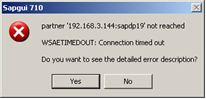
\includegraphics[scale=0.80]{../experiments/wp21-cr/ts01/SAP3.png}}
    \caption{\label{fig:SAP3}SAP message if the startup fails.}
\end{figure}

\paragraph{Shut Down}
%Describe the actions necessary to suspend testing, when unscheduled events dictate.
The test can be shut down by using the ''Exit'' entry in the GUI menu. In case that the system is not responding at all, the process kill options provided by Linux can be used. However, this might cause inconsistent data.

\paragraph{Restart}
%Identify any procedural restart points and describe the actions necessary to restart the procedure at each of
%these points.
A restart is only meaningful from the beginning. Thus, restart in this case means performing the test again right from the beginning.

\paragraph{Stop}
%Describe the actions necessary to bring execution to an orderly halt.
The WebAS can be stopped by using the ''Exit'' entry in the menu. In all other cases, the WebAS can be killed from the command line.

\paragraph{Wrap Up}
%Describe the actions necessary to restore the environment.
The test does not require an explicit wrap up. However, it is meaningful to remove the stored checkpoints after the test in order to keep the hard disc clean.

\paragraph{Contingencies}
%Describe the actions necessary to deal with anomalous events that may occur during execution.
In case of anomalies, the applications should simply be restarted.